\documentclass[class=scrartcl, crop=false,parskip=half]{standalone}
\usepackage[subpreambles=false]{standalone}
\usepackage{preamble}
\usepackage{import}


\begin{document}
%\section{Electromagnetic Radiation}\label{sec:emRadiation}
\subsection{Wave properties of EM radiation}
Solar energy makes use of some of the energy brought to us from the sun in the form of electromagnetic radiation.

James Clerk Maxwell showed in the 19th century that electric and magnetic fields can propagate together through a vacuum and through some transparent media as \emph{waves}. He convincingly showed that these waves travel through vacuum at the speed $c=\SI{2.997e8}{\metre\per\second}$, which was known by then to be the speed of light. In one of the great unifications of science, he had thus shown that light \emph{is} an electromagnetic wave. These waves are often referred to as electromagnetic waves, or EM radiation, and they exist across a continuous spectrum of wavelength, from  around a nuclear diameter $\SI{e-14}{\metre}$ at the short end to 1000s of km at the long end, a difference of 20 or so orders of magnitude. We make practical use in our modern lives of the whole of this spectrum. The part that is visible to us with our naked eye occupies a tiny sliver in the middle of this spectruim, with wavelengths ranging from about \SI{400}{\nm} (blue) to about \SI{700}{\nm} (red)

\begin{figure}
\centering
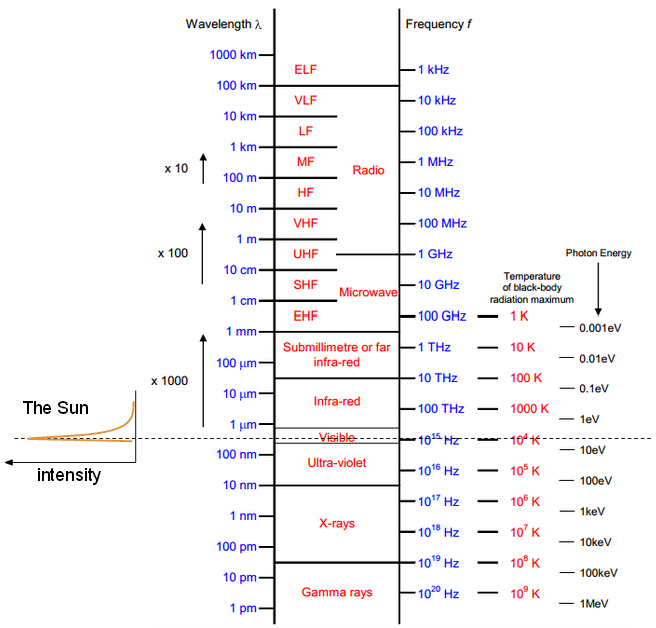
\includegraphics[width=\textwidth]{../figures/em-spectrum-with-sun.png}
\caption{The electromagnetic spectrum}
\label{fig:em-spectrum}
\end{figure}

Since EM radiation is a wave, it obeys the simple wave equation:

\begin{equation}
c=f\lambda
\label{eq:waveEquation}
\end{equation}
where $f$ is the wave frequency, $\lambda$ is the wavelength and $c$ is the wave speed. This equation is obeyed by all waves of whatever type, not just EM waves, but the distinguishing feature of EM waves that sets them apart from all others (such as sound waves, water waves and so on) is that $c$ is a constant for all observers, whatever their speed relative to the source of the radiation. $c$ is also very much faster than for  any other type of wave we encounter.  It's value in a vacuum is $c=\SI{2.997e8}{\metre\per\second}$. At this speed, light can cross the 150 million km between earth and the sun in a little over 8 minutes. In gases such as our atmosphere their speed is hardly different from this, but in other transparent media, such as water, glass, gem stones and some plastics, the speed of light is considerably slower than it is in a vacuum. The ratio of the speed of light in a vacuum to its speed in another medium is known as the \emph{refractive index} $\eta$ of the medium, and, given that light always travels more slowly in other media than it does in a vacuum, these values are always greater than one. For water, $\eta=1.333$, for glass, $\eta$ is in the range 1.46 to 1.69, while for diamond $\eta=2.4$. These and values for some other materials are collected together in Table \ref{tab:RefractiveIndices}.

\begin{equation}
\text{Refractive\ index\ of\ a\ medium}=\frac{\text{speed\ of\ light\ in\ vacuum}}{\text{speed\ of\ light\ in\ medium}};
\label{eq:refractive_index}
\end{equation}

\begin{table} 
\centering
\caption{Refractive index of some common transparent materials}
    \begin{tabular}{l l }
    \hline\\
    \textbf{Unit} & 	\textbf{Sun} \\
    \hline\\
    Water & 	1.333 \\
     \hline\\
    Glass& 	1.46-1.69 \\
    \hline\\
    Polycarbonate & 	1.58 \\
     \hline\\
    PET & 	1.57\\
    \hline\\
    Perspex & 	1.49\\
    \hline\\
    Diamond & 	2.4\\
    \hline\\
    \end{tabular}
\label{tab:RefractiveIndices}
\end{table}

EM waves are \emph{transverse} waves. This means that the electric and magnetic fields of which they consist oscillate in a direction perpendicular to the direction of travel of the wave rather than back and forth along that direction as longitudinal waves do, but the magnetic and electric field directions are always perpendicular to each other, as shown in Figure \ref{fig:em-wave}. 

\begin{figure}
\centering
\includegraphics[width=0.8\textwidth]{../figures/em-wave.tex}
\caption{A schematic of an electromagnetic wave. The wave is advancing in the $x$ direction, and consists of an oscillating electric field $E$ and magnetic field $B$, each of which is perpendicular to the other, and both are perpendicular to the direction of travel of the wave. Here they are shown oscillating in the $xy$ and $xz$ planes respectively. Sunlight is \emph{unpolarised} on arrival at the atmosphere, which means that along any beam, the $E$ and $B$ fields will be found oscillating in all planes around the direction of travel of the wave, not just the two shown here, but always be perpendicular to each other. }
\label{fig:em-wave}
\end{figure}

When they arrive at our atmosphere, EM waves from the sun are \emph{unpolarised}. That is, along a beam, the electric and magnetic fields are found oscillating in all possible directions perpendicular to the direction of travel of the wave, with short bursts in one direction followed by short bursts in another direction, as shown in Figure \ref{fig:unpolarised-light} . 

\begin{figure}
\centering
\includegraphics{../figures/unpolarised-light.tex}
%\\[0.5]
\caption{Bursts of unpolarised light travelling away from a source, showing only the electric field for clarity. From one burst to the next the electric field direction changes randomly, so that along the beam, it is found to be oscillating in all possible direction transverse to the direction of travel of the waves. Within any burst, the magnetic field direction is perpendicular to the electric field direction.}
\label{fig:unpolarised-light}
\end{figure}

In any one place, however, the two fields are always mutually perpendicular.  They can be \emph{linearly polarised} if passed through some special linear polarising materials that achieve this, and also by reflection off some surfaces, such as water and snow. Linearly polarised light has its magnetic field oscillating in one plane only, and the electric field in the plane perpendicular to that, as shown in Figure \ref{fig:linear-polariser}.

\begin{figure}
\centering
\includegraphics{../figures/Linear-polariser.tex}
%\\[0.5]
\caption{The action of a linear polarising filter on a beam of unpolarised light. The polariser has an axis, shown as an orange line, and lets through only the component of the incoming unpolarised beam whose electric field oscillates in the direction.}
\label{fig:linear-polariser}
\end{figure}

So, EM radiation is a transverse wave. As such it possesses the defining characteristics of any wave:
\begin{enumerate}
\item It will reflect off an interface between two media (eg air/glass, air/water) with a reflected angle equal to the angle of incidence, as shown in Figure \ref{fig:refraction}. 
\item Typically, a portion of the incident wave will also be transmitted through the medium, instead of being reflected. On entering the second medium, the light will slow down, as mentioned above, and this will cause it to change direction, a process known as \emph{refraction}. This can happen suddenly, where light passes from one medium to another and there is an abrupt change of speed and direction but whenever a wave changes speed it will in general change direction. This is what causes shallow water sea waves, which travel more slowly the shallower the water becomes, to veer towards the shore and approach the beach more or less parallel to it, no matter where they originally came from.

\begin{figure}
\centering
\includegraphics[width=0.5\textwidth]{../figures/refraction.tex}
\caption{A beam of light incident upon an air-water interface is partially reflected and partially transmitted.}
\label{fig:refraction}
\end{figure}
\item The proportion that is reflected or transmitted can change from almost 100\% of one to almost 100\% of the other, depending on the angle of incidence, as shown in Figure \ref{fig:reflectivity}. When light strikes water or glass  from air, for example, 96\% of it is transmitted at normal (ie straight down) incidence, whereas virtually all is reflected at grazing (ie virtually parallel with the water/glass surface) incidence. This is an important consideration when estimating the energy that solar collector will trap over a day, during which the sun will move and the angle of incidence will change. Sunlight that reflects from the surface of the collector is energy lost!
\begin{figure}
\centering
%[width=\textwidth]
\includegraphics[width=0.8\textwidth]{../figures/reflectivity.tex}
\caption{Variation with angle of incidence of the proportion of light incident upon a glass surface, from air, that is reflected and transmitted.}
\label{fig:reflectivity}
\end{figure}
\item it displays \emph{interference} and \emph{diffraction} effects. These properties become prominent when the wavelength of the wave is comparable to other sizes in the system, but visible light waves have a wavelength of fractions of a micrometer, and so diffraction and interference of visible light plays little role in solar energy collectors.
\end{enumerate}
\subsection{EM radiation as photons}
The wave model of EM radiation  explains many phenomena very well, but was first shown by Planck and Einstein in the early 20$^{\text{th}}$ century to be incomplete. Einstein sought to understand the \emph{photoelectric effect}, in which electric current is emitted from the surface of metals when ultra-violet light is shone upon it. When the metal is zinc, so-called photo-electrons are emitted when the incident radiation is UV, but none are emitted when visible light is used instead, no matter how intense the light source.
Einstein showed that this can be explained if we realize that, while light and every other part of the EM spectrum certainly display wave like behaviour, it \emph{also} is a stream of particles, now called \textbf{photons}. How it can be both a wave and a stream of particles is very difficult for us to imagine, but the efforts and experimental results of the more than 100 years since the pioneering work of Planck and Einstein strongly suggests that this is because our imagination is limited, not because it isn't true.

Einstein showed that the energy of these photons (if we think of light as a stream of particles) is proportional to the frequency of the wave (if we think of light as a wave), with the constant of proportionality being the Planck constant $h=\SI{6.6e-34}{\joule\second}$
\begin{equation}
E=hf=\dfrac{hc}{\lambda}
\label{eq:hf}
\end{equation}
where $f$ is the frequency of the wave and $c$ is its speed. Actual photon energies are very small numbers if we use the SI unit joule. A more convenient unit that is widely used is the electron volt (eV) or its multiples keV and MeV. 
\begin{equation}
\SI{1}{eV}=\SI{1.602e-19}{\joule}
\label{eq:eV}
\end{equation}
In this unit, the energy of visible light photons range from about 3.1 eV (blue) to 1.77 eV (red). UV light has higher photon energies, and infra-red light has lower photon energies.

For solar energy purposes, a handy way to find the photon energy of a given part of the spectrum is given by
\begin{equation}
\text{photon energy in eV}=\dfrac{1240}{\text{wavelength in nm}}
\label{eq:eV2}
\end{equation}

\end{document}
